\section{Distances}
\frame{
    \frametitle{}

\begin{block}{}
    \centering
    Distance Measures:\\
    Comparing Descriptors
\end{block}
}

\frame{
\frametitle{}

\begin{block}{}
\centering
 \only<1>{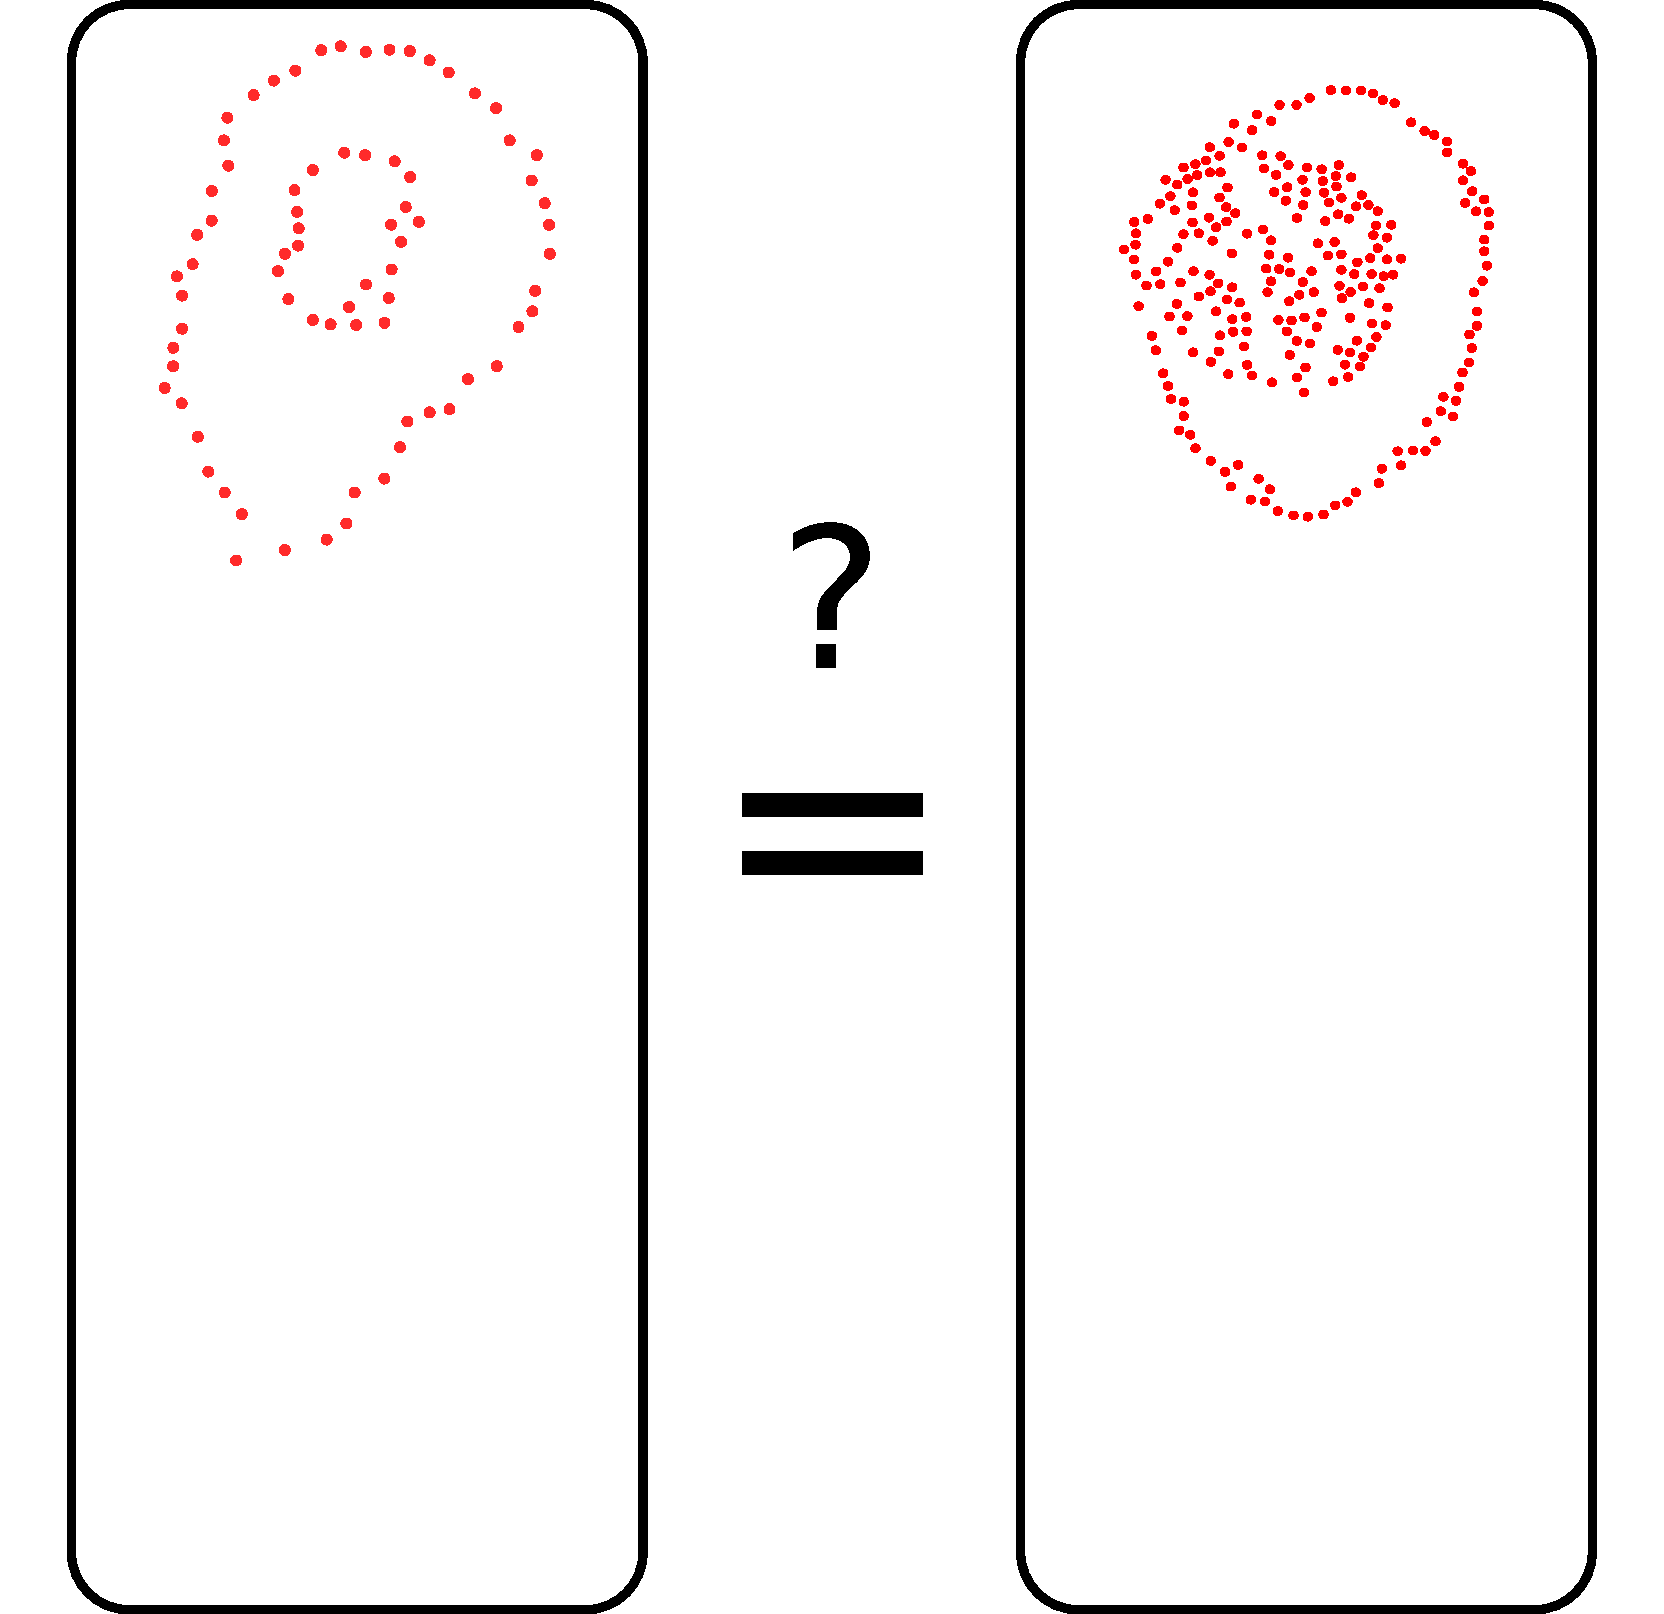
\includegraphics[width=.7\textwidth]{topology/inference-compare-1}}%
 \only<2->{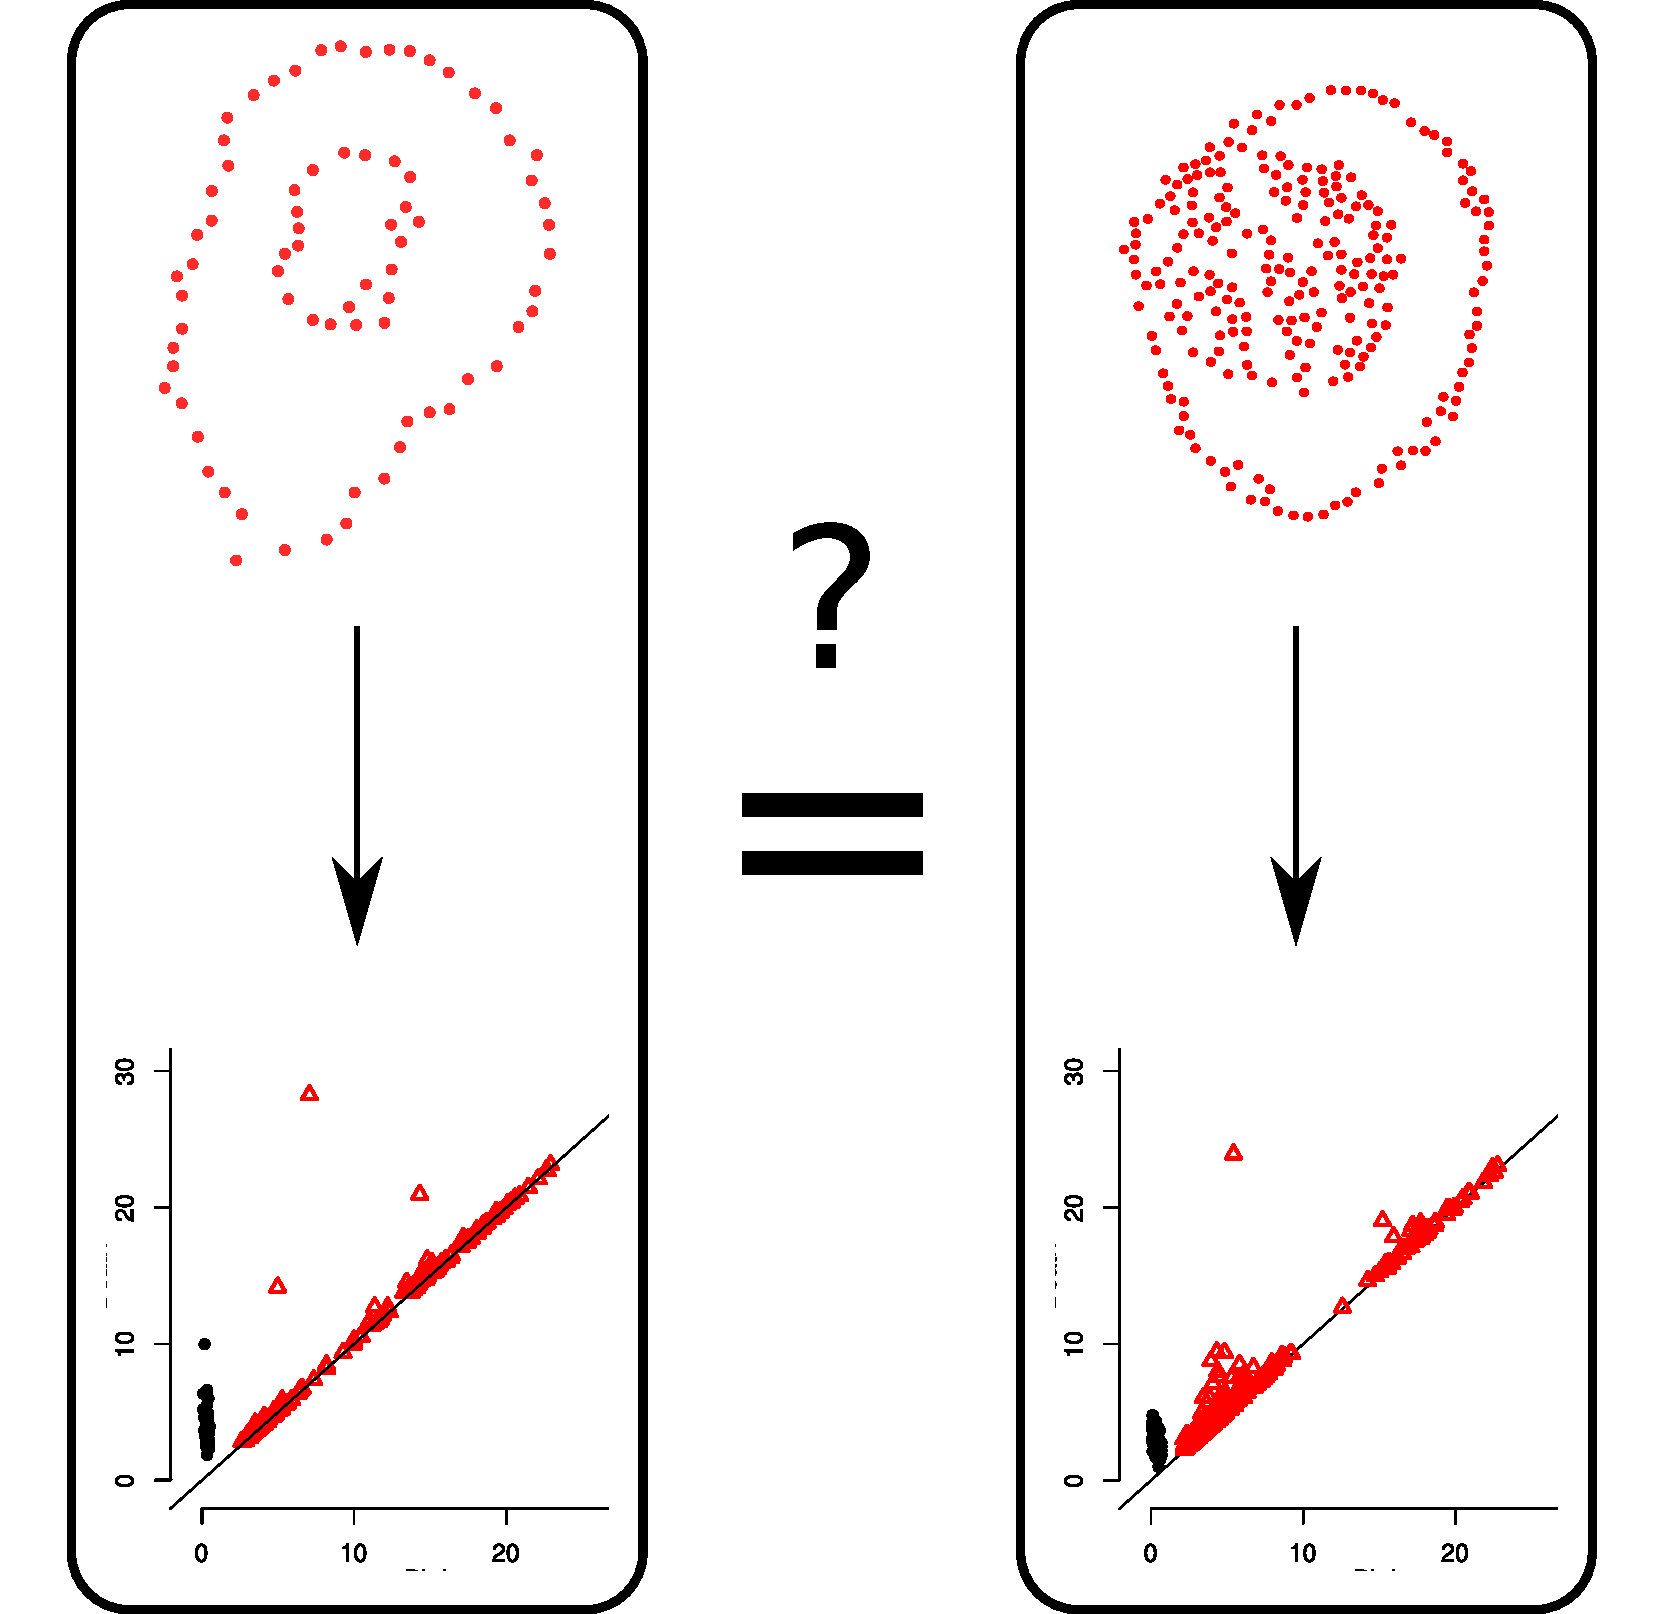
\includegraphics[width=.7\textwidth]{topology/inference-compare-2}}%
\end{block}

}


\frame{
    \frametitle{Distances Between Diagrams}
    \begin{columns}%
        \column{.45\textwidth}
        \begin{block}{}
            \onslide<1->{
                \begin{itemize}
                    \item Bottleneck $d_{\infty}$.
                    \item Interleaving distance.
                    \item Wasserstein $d_p$.
                    \item Erosion distance.%
                \end{itemize}%
            }%
        \end{block}%
%
        \pause%
        \begin{block}{Question}%
            Can we define a centroid / Fr\'echet mean?
            $$ \arg\min_D \sum_i W^2_{\infty}(D,D_i)$$
        \end{block}%
%
            \pause
            \column{.45\textwidth}
        \begin{block}{}
            \centering
            \only<2>{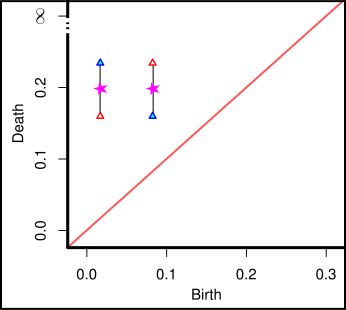
\includegraphics[height=1.9in]{stat/dgm-average}}%
            \only<3>{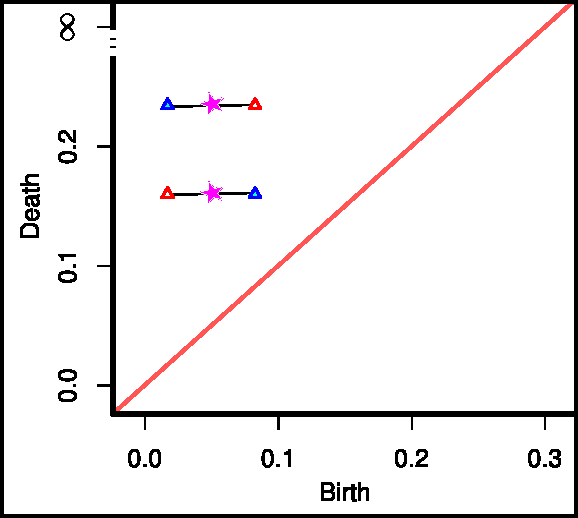
\includegraphics[height=1.9in]{stat/dgm-average-opt1}}%
            \only<4->{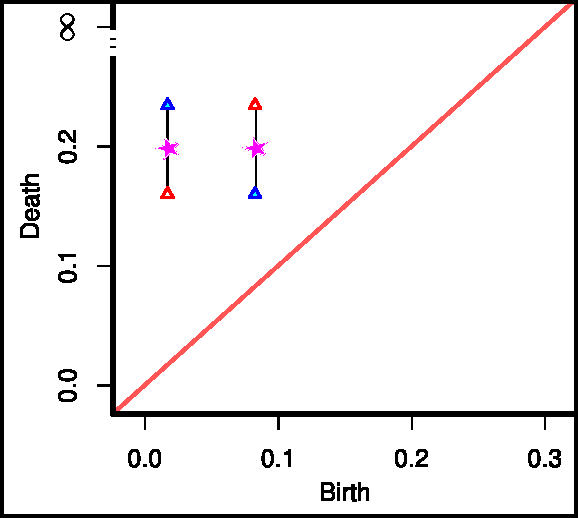
\includegraphics[height=1.9in]{stat/dgm-average-opt2}}%
        \end{block}

        \tiny{
        1. Turner, Mileyko, Mukherjee, and Harer. Fr\'echet Means for Distributions
        of Persistence Diagrams. DCG, 2014.\\
        2. Munch, Tuner, Bendich, Mukherjee, Mattingly, and Harer.
        Probabilistic Fr\'echet Means for Time Varying Persistence Diagrams.
        Electronic Journal of Statistics, 2015.
    }

    \end{columns}
}

\frame{
\begin{block}{}
\centering
 \only<1>{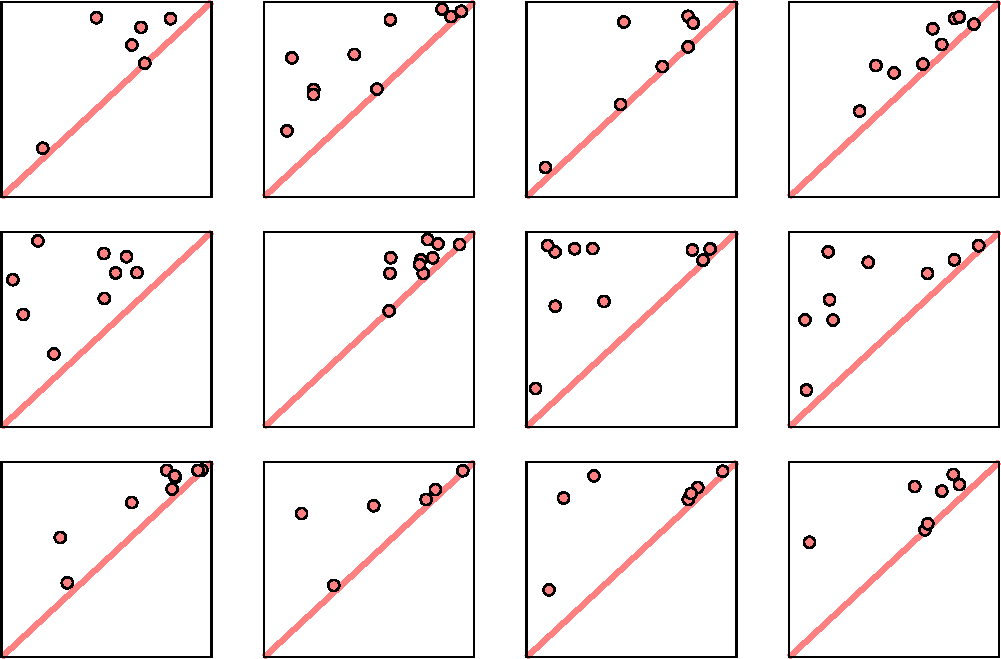
\includegraphics[width=.7\textwidth]{stat/sampling-dgms}}%
 \only<2->{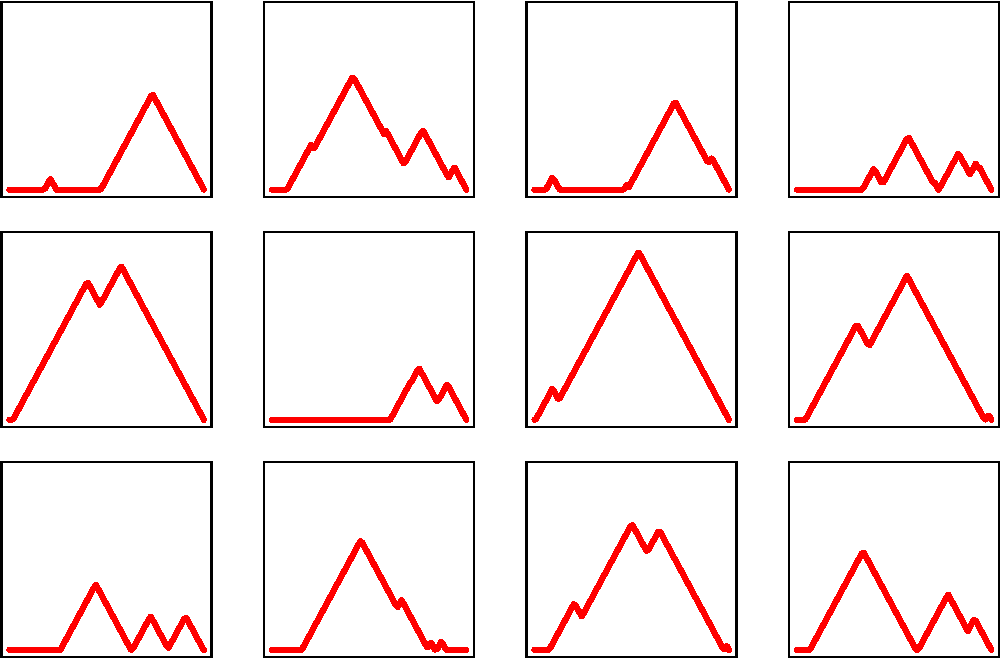
\includegraphics[width=.7\textwidth]{stat/sampling-lscapes}}%
\end{block}

}

\frame{

\begin{block}{}
    \centering
   Clustering
\end{block}
}

\frame{
    \frametitle{Clustering
    \onslide<5->{... and Classification} }

    \begin{block}{Clustering (Unsupervised Learning)}
        \pause
        \begin{itemize}
            \item Heirarchical: agglomerative or divisive.\pause
            \item $k$-means: NP-hard, so algorithms find a local minimum.
            \item Distribution- and density-based clustering: e.g., DBSCAN.
                \pause
            \item Fuzzy clustering: membership is not binary.
        \end{itemize}
    \end{block}

    \pause%
    \begin{block}{Classification (Supervised Learning)}
        input data (training sample): $D=\{(X_i,Y_i)\}_{i=1}^n$\\~\\
        $k$-nn clustering: for new $X$, we predict $Y$ by majority vote of the
        $k$ nearest neighbors of the covariates (features) in $D$.
    \end{block}
}
